\hypertarget{Design}{\chapter{Design}}

\section{Motivace}

Při tvorbě aplikace bylo neustále nutné myslet na dva hlavní faktory, kolem kterých se celý design musí odvíjet; to sice, že je program mířený pro dvě skupiny: učitele a žáky zároveň. 

Úkolem žáka je v testu odpovídat na otázky. Žák by měl mít co nejméně možností, jak podvádět, aby byl správně umístěn do jazykové skupiny úměrné jeho znalostem; dostane náhodnou podmnožinu otázek různých obtížností, které pro jeho ročník navolí učitel.

Učitel pracuje se svým vlastním rozhraním, kde zadává otázky, vytváří testy, kontroluje průběh testování a získává automaticky zpracované výsledky.

V obou případech je důležité, aby byla webová aplikace intuitivní na používání, měla příjemný design a hlavně spolehlivě fungovala.

\section{Přihlašování}

Ještě před tím, než se uživatelé dostanou do svého rozhraní, je potřeba, aby se přihlásili. Tato část aplikace je společná pro žáky i učitele. 

\begin{figure}[H]
    \centering
    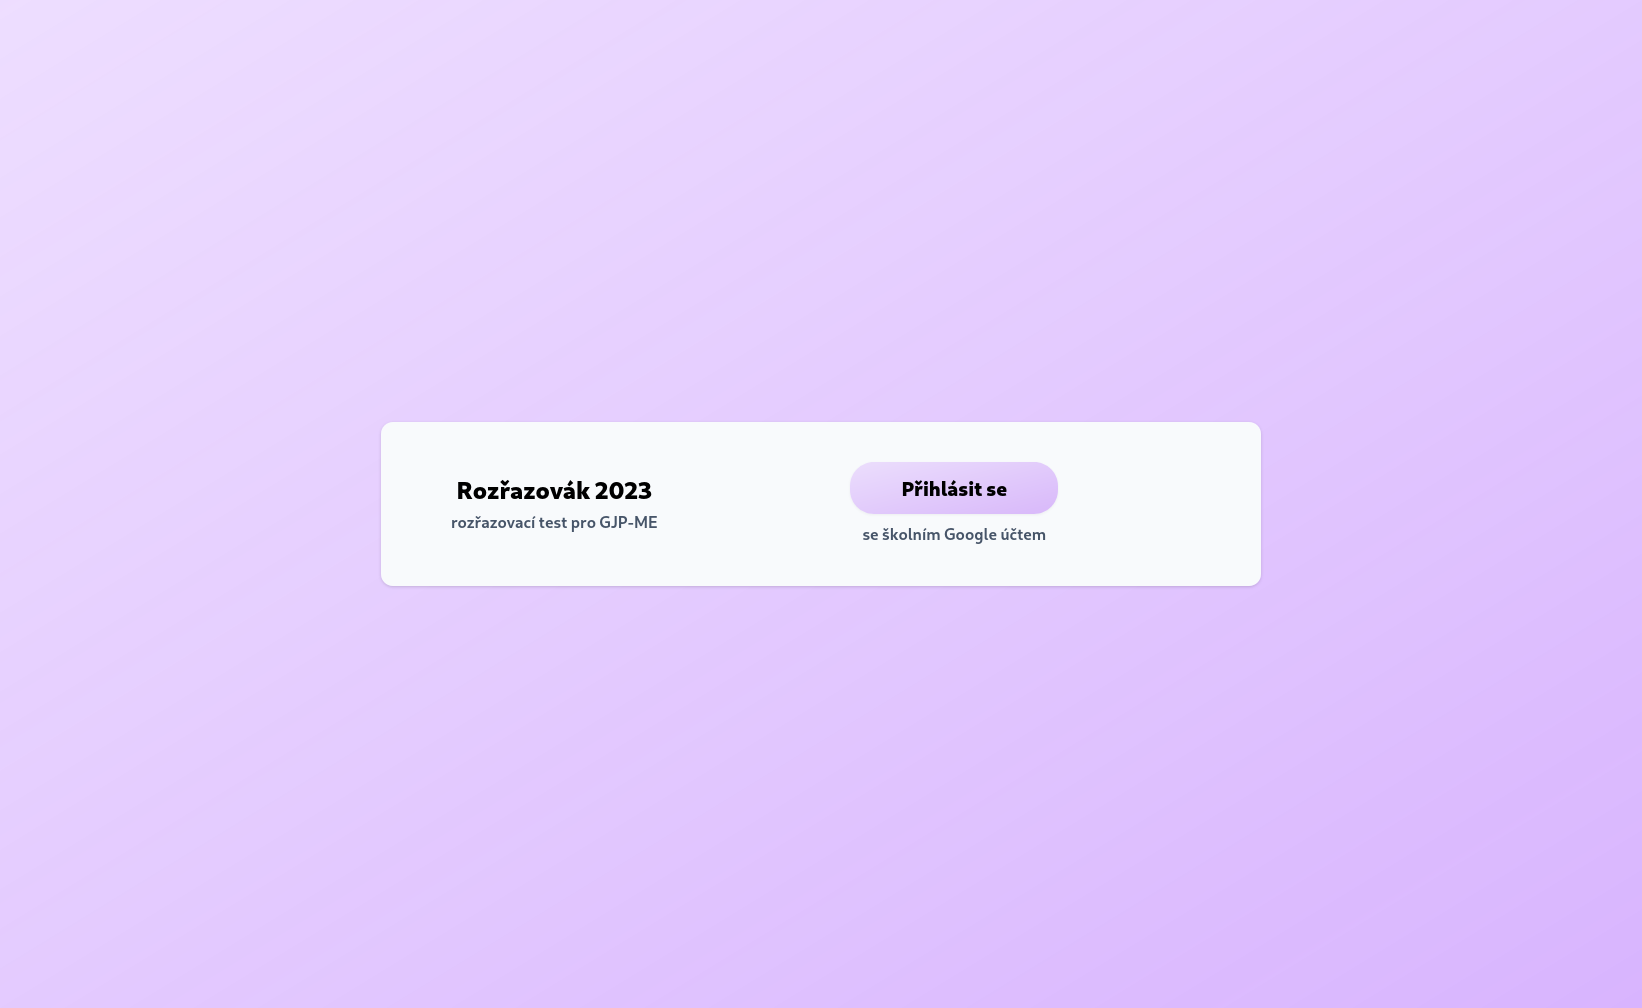
\includegraphics[width=350px]{images/01design/login.png}
    \caption{Přihlašovací stránka je hlavní stránkou aplikace.}
\end{figure}

Učitelé a žáci se přihlásí pomocí svého školního Google účtu (vizte kapitola 2.X.X).

\newpage

Pokud se přihlásí učitel, zobrazí se mu nabídka pro přechod do administrátorské sekce.

\begin{figure}[H]
    \centering
    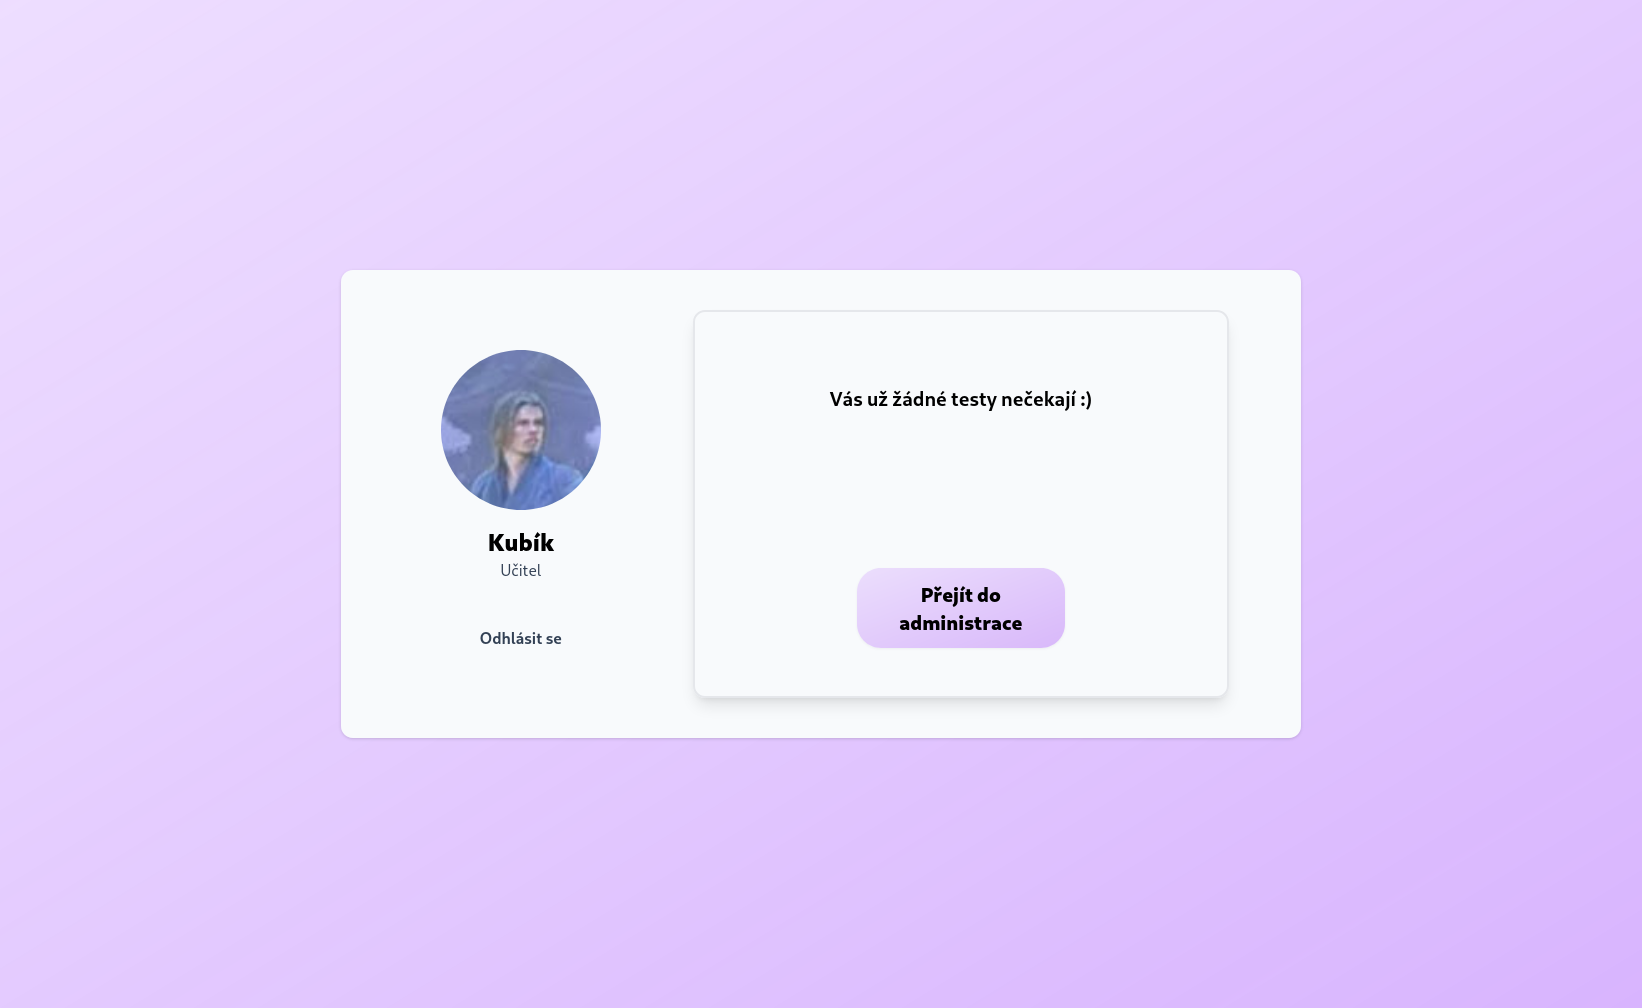
\includegraphics[width=350px]{images/01design/teacher.png}
    \caption{Hlavní stránka po přihlášení učitele.}
\end{figure}

Pokud se přilhásí žák, záleží na tom, zdali je pro jeho ročník aktuálně spuštěný test. Pokud ne, zobrazí se pouze informace o tom, že pro žáka žádný test aktuálně spuštěný není; pokud ano, zobrazí se informace o jeho trvání a počtu otázek, spolu s možností test spustit.

\begin{figure}[H]
    \centering
    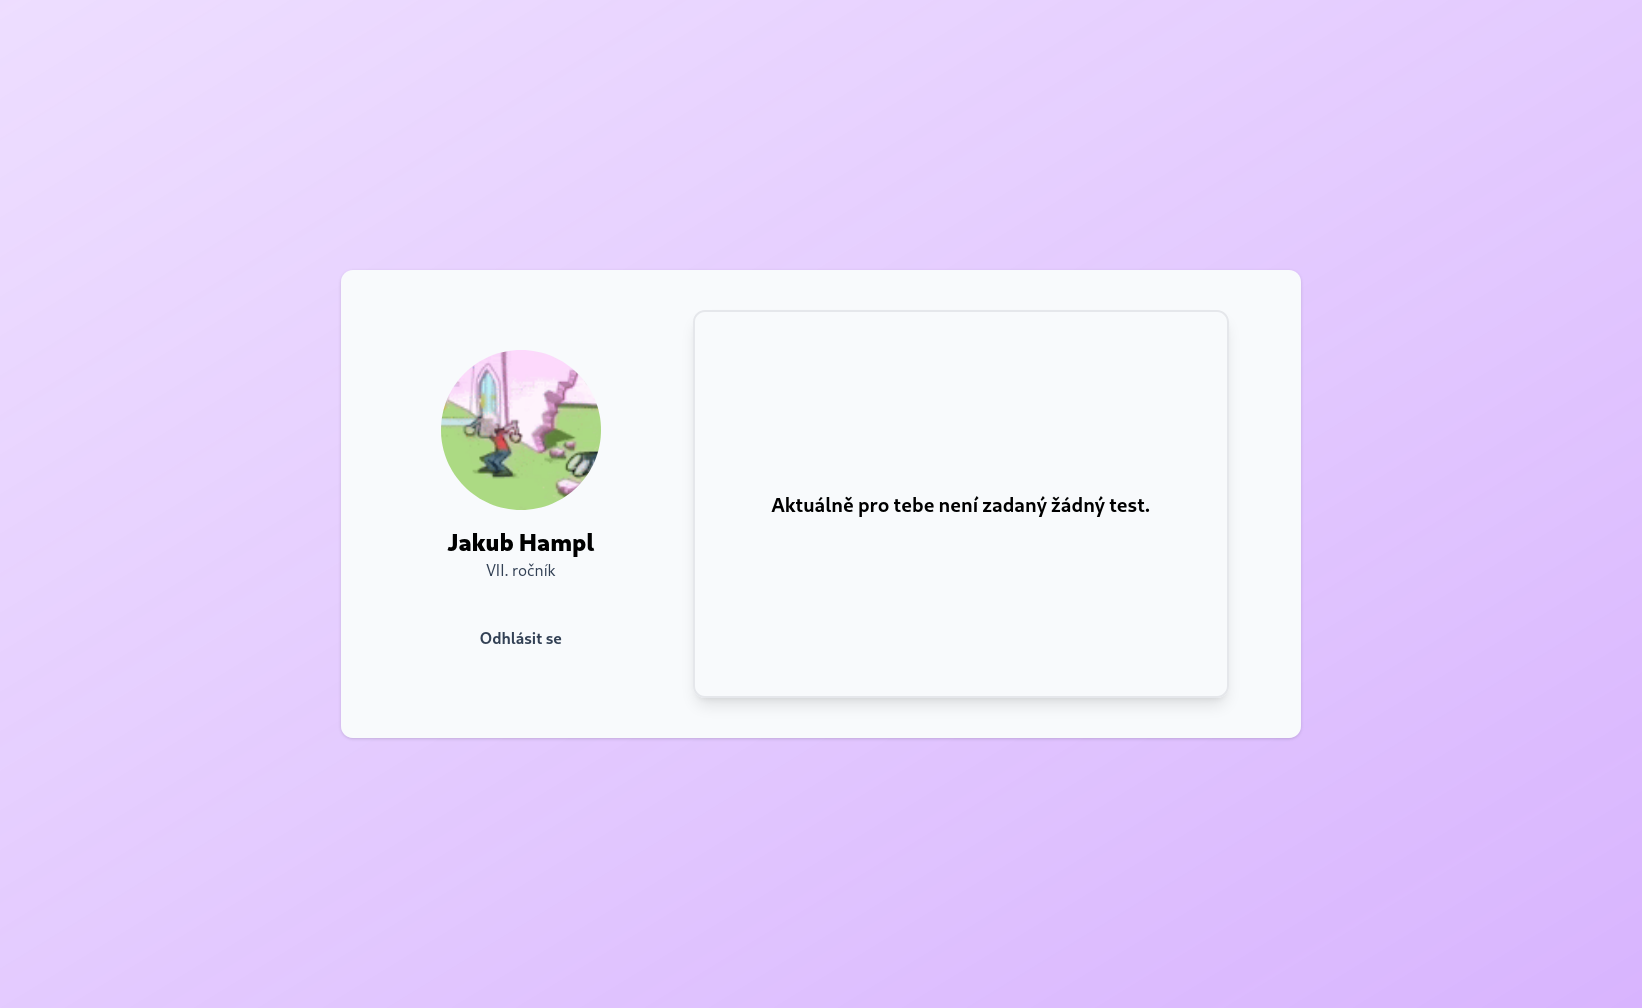
\includegraphics[width=350px]{images/01design/student-no-test.png}
    \caption{Hlavní stránka po přihlášení žáka bez zadaného testu.}
\end{figure}

\section{Žákovské rozhraní}

Žákovské rozhraní slouží k vyplňování zadaných testů. Po přihlášení je přesměrován do rozhraní, kde jsou pro něj vygenerované otázky (vizte kapitola 2.X.X). Žák má na výběr ze čtyř možností z nihž je vždy pouze jedna správně.

\section{Učitelské rozhraní}